% ============================================================
%  Temporal Partial Information Decomposition of EEG During Sleep
%  Short-window pass (1-second resolution) -- Technical Report
%  Compile with pdflatex.
% ============================================================
\documentclass[11pt,a4paper]{article}

\usepackage[margin=2.5cm]{geometry}
\usepackage{amsmath,amssymb}
\usepackage{graphicx}
\usepackage{booktabs}
\usepackage{array}
\usepackage{caption}
\usepackage{subcaption}
\usepackage[colorlinks=true,linkcolor=blue,citecolor=blue,urlcolor=blue]{hyperref}
\usepackage{microtype}
\usepackage{xurl}
\usepackage{parskip}
\usepackage{xcolor}
\usepackage{siunitx}

\usepackage{natbib}
\bibliographystyle{plainnat}

\title{\textbf{Temporal Partial Information Decomposition\\of Human EEG Across Sleep Stages}\\[4pt]
\large Short-window pass (1-second resolution)}
\author{Temporal Information Decomposition Project}
\date{June 2026}

% ============================================================
\begin{document}
\maketitle
\tableofcontents
\newpage

% ============================================================
\section{Abstract}
% ============================================================

We apply \emph{Temporal Partial Information Decomposition} (Temporal PID) to
overnight polysomnography EEG from 10 healthy adults to characterise how the
information structure of cortical dynamics changes across sleep stages.
For every 1-second EEG window we construct temporal triplets at pairs of
second-scale lags ($\tau_1, \tau_2 \in [1, 30]$~s) and decompose the predictive
information about the target window into four atoms: \emph{redundancy},
\emph{synergy}, \emph{unique information from the shorter lag} (Unique$_1$),
and \emph{unique information from the longer lag} (Unique$_2$), using the
Minimum Mutual Information (MMI) PID measure.
The first 3.5 hours of each recording are analysed, sufficient for two
NREM--REM cycles and per-stage AR(1) fits.
All four atoms show highly significant stage-dependent variation
(Kruskal--Wallis $p < 10^{-25}$, pooled across electrodes), with the largest
effect sizes concentrated in slow-wave sleep (N3) for redundancy and total
unique information.  A within-stage variability analysis shows that N3 has
the lowest coefficient of variation on redundancy and total unique
information while simultaneously having the highest mean, identifying it as
a coherent, low-variance multi-timescale state.  A band-resolved analysis
on three subjects reveals an $\alpha$ versus $\delta$ inversion of the
synergy-to-redundancy ratio across stages, an effect that is hidden by
broadband averaging.

% ============================================================
\section{Introduction}
% ============================================================

Sleep staging traditionally rests on spectral features such as slow-wave power,
sleep spindle density, and K-complex count~\citep{berry2012aasm}.  These
measures capture \emph{linear, single-timescale} properties of the EEG.  The
rich temporal dynamics of sleep, characterised by travelling slow oscillations
that coordinate memory consolidation, hippocampal sharp-wave ripples, and
thalamo-cortical spindles, involve \emph{multi-timescale, non-linear}
interactions that spectral power alone cannot resolve.

Partial Information Decomposition (PID)~\citep{williams2010nonnegative} is an
information-theoretic framework that decomposes the total predictive
information shared between a set of source variables and a target into
non-negative, non-overlapping atoms: information carried \emph{redundantly} by
all sources, information \emph{unique} to each source, and information
available only when sources are considered \emph{jointly} (synergy).  When
applied across temporal lags (comparing a signal to its own past at two
different delays), PID quantifies the temporal self-predictability structure
of neural dynamics: redundancy captures stable periodic or auto-correlated
features, synergy captures joint predictive structure across lag pairs not
visible at any single lag, and unique information measures lag-specific
predictability.

In this report we apply Temporal PID to broadband EEG from an overnight
polysomnography dataset at the second timescale.  We quantify how each atom
varies across the five standard sleep stages (Wake, N1, N2, N3, REM), test
statistical significance via block-permutation, and split the broadband
analysis into five frequency bands ($\delta$, $\theta$, $\alpha$, $\sigma$,
$\beta$) to localise the spectral origin of the stage signature.

% ============================================================
\section{Methods}
% ============================================================

\subsection{Dataset and participants}

EEG data were taken from OpenNeuro \texttt{ds005555} (10 healthy adults,
overnight polysomnography).  The first 3.5~hours of each recording were
analysed, capturing two full NREM--REM cycles.  Six scalp channels (F3, F4,
C3, C4, O1, O2) were loaded with MNE-Python~\citep{gramfort2013meg}; sleep
stages were read from the accompanying \texttt{*psg\_events.tsv} files (AASM
five-class system).

Figure~\ref{fig:method} provides an overview of the full pipeline.

\begin{figure}[tbp]
  \centering
  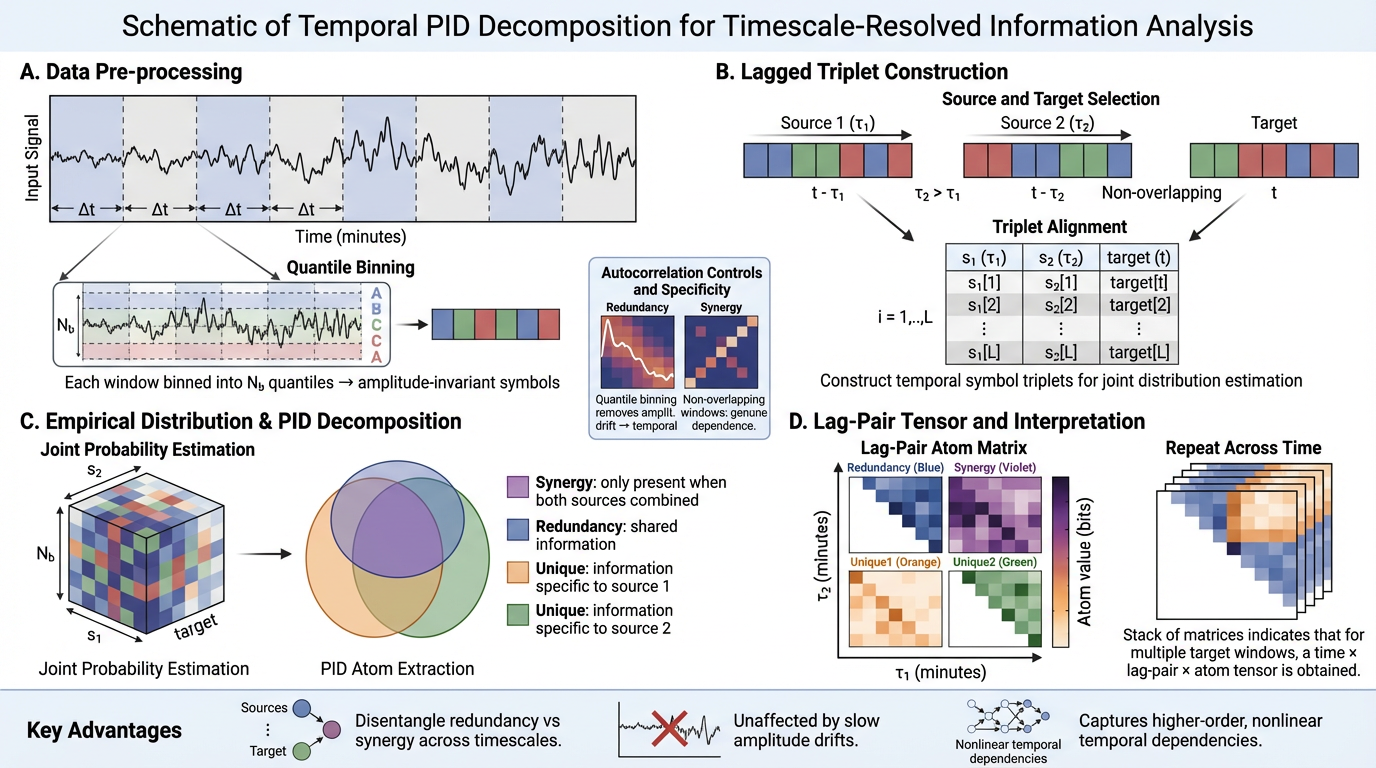
\includegraphics[width=\textwidth]{../docs/Temporal-PID_figure.png}
  \caption{%
    \textbf{Overview of the Temporal PID pipeline.}
    (A)~Input signal segmented into fixed-length windows ($\Delta t = 1$~s)
    and independently discretised into $N_b = 4$ quantile bins, producing
    amplitude-invariant symbol sequences.
    (B)~Lagged triplet construction: for each target window $t$, two past
    windows at offsets $\tau_1 < \tau_2$ are aligned sample-by-sample to form
    the source--target triplet
    $(\mathbf{s}_1, \mathbf{s}_2, \mathbf{x}(t))$.
    (C)~The empirical joint distribution over the $N_b^3 = 64$ symbol states
    is estimated by co-occurrence counts; PID with the MMI measure decomposes
    it into four non-negative atoms (redundancy, synergy, unique$_1$,
    unique$_2$).
    (D)~Repeating the decomposition across all 435 lag pairs
    $(\tau_1, \tau_2)$ and all valid target windows yields a
    time $\times$ lag-pair $\times$ atom tensor.
  }
  \label{fig:method}
\end{figure}

\subsection{Preprocessing}

Each EEG channel was:
\begin{enumerate}
  \item Bandpass filtered (0.5--60~Hz, 4th-order Butterworth, zero-phase);
  \item Notch filtered at 50~Hz and 60~Hz (IIR notch, $Q = 30$) to remove
        power-line interference.
\end{enumerate}
No amplitude normalisation was applied at this stage.

\subsection{Windowing and Discretisation}

The continuous signal was divided into non-overlapping windows of
$\Delta t = \SI{1}{\second}$, yielding $N_w = \lfloor T / \Delta t \rfloor$
windows.  Each window was independently discretised into $N_b = 4$ levels
using \emph{quantile binning}: bin edges were computed from the empirical
percentiles of that window alone, so that each bin contains approximately the
same number of samples.  $N_b = 4$ provides the joint distribution
$p(\mathbf{s}_1, \mathbf{s}_2, \mathbf{x})$ with $4^3 = 64$ cells against
the $\Delta t \times f_s = 256$ samples available per triplet, which keeps
the per-cell sample count in the regime where the empirical estimator
behaves reasonably.

Per-window discretisation is critical: it renders the analysis
amplitude-invariant within a window and removes slow power drifts at the
window timescale, so that information-theoretic measures capture temporal
\emph{pattern} rather than amplitude covariation.

\subsection{Temporal Triplet Construction}

For a target window $\mathbf{x}(t)$ and two lag offsets $\tau_1 < \tau_2$
(in seconds), the temporal triplet is:
\begin{equation}
  \bigl(\mathbf{s}_1,\, \mathbf{s}_2,\, \mathbf{x}(t)\bigr)
  = \bigl(\mathbf{x}(t - \tau_1),\, \mathbf{x}(t - \tau_2),\, \mathbf{x}(t)\bigr).
\end{equation}
The three vectors are aligned sample-by-sample within each window, yielding
$L = \Delta t \times f_s = 256$ co-occurring symbol triples per triplet
formation.  Lag offsets were set on a 1-second grid from 1 to 30~seconds
($\tau \in \{1, 2, \ldots, 30\}$~s), producing $\binom{30}{2} = 435$ distinct
lag pairs $(\tau_1, \tau_2)$ with $\tau_1 < \tau_2$.

The time-resolved PID is evaluated on a strided target axis with
\texttt{TARGET\_STEP} $= 3$ (one estimate every 3~s).  Each estimate still
uses the full 1-second target and source windows; only the time-axis density
of estimates is thinned.  The global PID matrix and the AR(1) baseline are
unaffected.

\subsection{PID Decomposition}

The empirical joint distribution $p(\mathbf{s}_1, \mathbf{s}_2, \mathbf{x})$
over $N_b^3 = 64$ states was estimated by counting co-occurrences.
\emph{Partial Information Decomposition} with the Minimum Mutual Information
(MMI) measure~\citep{barrett2015exploration} was then applied, yielding the
four non-negative atoms:
\begin{align}
  R &= \min\!\bigl(I(\mathbf{s}_1;\mathbf{x}),\, I(\mathbf{s}_2;\mathbf{x})\bigr), \\
  U_i &= I(\mathbf{s}_i;\mathbf{x}) - R, \\
  S &= I(\{\mathbf{s}_1,\mathbf{s}_2\};\mathbf{x})
      - I(\mathbf{s}_1;\mathbf{x}) - I(\mathbf{s}_2;\mathbf{x}) + R.
\end{align}
This closed form is mathematically equivalent to the lattice-walking
\texttt{PID\_MMI} routine in the \texttt{dit}
library~\citep{james2018dit}; the two were verified to agree to
$10^{-15}$ across IID, COPY, XOR, and AR-correlated test cases.  At
256-sample joints the closed form is roughly $10^3$ times faster per call
than the \texttt{dit} reference, which makes the per-window pass feasible.

\begin{table}[h]
\centering
\caption{PID atoms and their temporal interpretation.}
\label{tab:atoms}
\begin{tabular}{@{}lp{9cm}@{}}
\toprule
\textbf{Atom} & \textbf{Temporal interpretation} \\
\midrule
Redundancy~$R$ & Predictive information about $\mathbf{x}(t)$ carried
  \emph{independently} by both past windows; reflects stable periodic or
  auto-correlated structure consistent across multiple timescales. \\[4pt]
Synergy~$S$ & Predictive information available \emph{only} when both past
  windows are considered jointly; captures joint predictive structure across
  lag pairs not visible at any single lag, consistent with but not solely
  diagnostic of cross-timescale interactions. \\[4pt]
Unique$_1$~$U_1$ & Predictive information carried exclusively by the
  shorter-lag source $\mathbf{s}_1$; measures the added value of recent
  history. \\[4pt]
Unique$_2$~$U_2$ & Predictive information carried exclusively by the
  longer-lag source $\mathbf{s}_2$; measures the added value of more distal
  history. \\
\bottomrule
\end{tabular}
\end{table}

The four atoms partition the total predictive information:
\begin{equation}
  I\!\left(\{\mathbf{s}_1, \mathbf{s}_2\}; \mathbf{x}(t)\right)
  = R + S + U_1 + U_2.
\end{equation}

Two complementary summary statistics are reported.  The
\textbf{synergy-to-redundancy ratio} $S/R$ measures whether multi-lag
temporal structure is dominated by joint predictive information; values
$> 1$ indicate synergy exceeds redundancy.  For confound checks and
timescale analyses we additionally report the \textbf{normalised ratio}
$S/(S + R) \in [0, 1]$, which is amplitude-invariant across stages with
different absolute PID magnitudes.

\subsection{Stage Filtering and Coverage Correction}

A temporal triplet $(\tau_1, \tau_2, t)$ was retained for stage $k$ only if
\emph{every window in the span from $t - \tau_2$ to $t$} was scored as stage
$k$.  Because the hypnogram is scored in 30-second blocks and the maximum
lag is 30~s, this guarantees the triplet lies entirely within one 30-s
scored bout and cannot straddle a stage transition.

Because sleep stages differ in bout duration (N3 bouts can exceed 30~min;
N1 seldom exceeds 3~min), different stages yield different subsets of
available lag pairs.  Naively averaging over all available pairs would
create a \emph{coverage bias}: shorter stages would contribute only
short-lag (high-information) pairs and therefore appear artificially
elevated.  To correct this, all cross-stage comparisons restrict to the
\textbf{common lag range}, the intersection of $(\tau_1, \tau_2)$ pairs
that are present in \emph{every} stage, so that per-window means are
computed over identical timescale subsets.

\subsection{Stage-conditional AR(1) baseline}
\label{sec:methods:ar1}

A sample-level AR(1) process is fit \textbf{per sleep stage}: the
coefficient $\phi$ and noise $\sigma$ are estimated on that stage's
discretised windows alone (minimum 20 windows per stage; otherwise the
stage is excluded from the fit).  A synthetic AR(1) PID matrix is generated
per stage and broadcast to each target window according to its stage label.
The \emph{excess} (Actual $-$ stage-AR(1)) is then a within-stage measure
of non-linear or higher-order temporal structure, isolated from across-stage
spectral differences.

\subsection{Band-resolved analysis}
\label{sec:methods:bands}

To check whether the broadband patterns reflect a band-specific signature
or a mixed contribution, the full pipeline is also run after
bandpass-filtering the signal into five standard frequency bands:
$\delta$ 0.5--4~Hz, $\theta$ 4--8~Hz, $\alpha$ 8--13~Hz, $\sigma$ 11--16~Hz,
and $\beta$ 16--30~Hz (Butterworth 4th order, zero-phase).  All other
parameters are identical to the broadband pass.  To bound wall-time the
band-resolved pass is run on 3 subjects $\times$ 6 channels = 18
(subject $\times$ channel) units per band, against the 60 units of the
broadband pass.

\subsection{Statistical Testing}

\subsubsection{Group-level stage comparison}

For each subject, electrode, and lag pair, the per-window PID atoms were
averaged within each stage.  The resulting per-window means (pooled across
all 10 subjects and all common lag pairs) were compared across the five
stages using the non-parametric \textbf{Kruskal--Wallis} (KW) test.
Pairwise post-hoc comparisons used the \textbf{Mann--Whitney U} test with
Benjamini--Hochberg false-discovery-rate (BH-FDR)
correction~\citep{benjamini1995fdr} applied across all $\binom{5}{2} = 10$
stage pairs.

\subsubsection{Block-permutation test for lag-pair significance}
\label{sec:blockperm}

To test whether PID at each lag pair $(\tau_1, \tau_2)$ exceeds chance
temporal structure, we applied a \textbf{block-permutation} null: the
1-second EEG window was treated as the atomic block, and a uniform random
permutation of window indices was applied to the full recording ($n = 100$
surrogates per subject), preserving within-window waveform and amplitude
structure while destroying all cross-window temporal ordering at every
tested lag scale ($\tau \geq 1$~s).  The empirical $p$-value is the
fraction of surrogates exceeding the observed statistic; the heatmaps in
Figure~\ref{fig:block_perm} show the group-mean $-\log_{10}(p)$, with
asterisks marking lag pairs where $p < 0.05$.  At a block size of 1~s the
shuffle destroys nearly all linear autocorrelation at the tested lag
range, so atoms surviving the shuffle reflect structure on the
sub-second / within-window scale.

To bound wall-time, the block-permutation null was computed only for the
\textbf{C3 composite}; per-subject per-channel block-perm at 1-s windows
is the dominant cost in the pipeline and is dropped here without loss
because the figure was already group-level C3 only in the broader
literature.

% ============================================================
\section{Results}
% ============================================================

\subsection{PID dynamics across the night}

Figure~\ref{fig:timeseries} illustrates the evolution of Temporal PID across
a 3.5-hour recording for a representative subject (sub-1, electrode C3).
Each trace panel shows the mean PID atom (pooled over all lag pairs) for
every target window at the 3-second \texttt{TARGET\_STEP} resolution; the
top panel shows the concurrent hypnogram.  All three atoms track sleep-stage
identity in real time: redundancy and synergy are markedly elevated during
N3 blocks and drop when the recording transitions to lighter stages or REM.

\begin{figure}[tbp]
  \centering
  \includegraphics[width=\textwidth]{%
    ../results/pid/eeg_sleep/PID-10-subjects-1sec/sub-1/C3/hypnogram_pid_timeseries_ba79f4ef.png}
  \caption{%
    \textbf{Temporal PID time series across the recording (sub-1, C3,
    representative).}
    Top: hypnogram with stage-coloured background bands.  Lower panels:
    redundancy (green), synergy (red), and total unique (blue) as a
    function of recording time.  Each trace is the mean across all 435
    lag pairs; the 25--75\% range across lag pairs is shown as a shaded
    band.
  }
  \label{fig:timeseries}
\end{figure}

\subsection{Stage-dependent PID structure}

Figure~\ref{fig:stage_comparison} shows boxplots of all four PID atoms and
the synergy-to-redundancy ratio, pooled across all six electrodes and all
10 subjects, stratified by sleep stage.

\begin{figure}[tbp]
  \centering
  \includegraphics[width=\textwidth]{%
    ../results/pid/eeg_sleep/PID-10-subjects-1sec/group/group_all_stage_comparison_ba79f4ef.png}
  \caption{%
    \textbf{PID atoms by sleep stage, group-level (n = 10 subjects, all
    electrodes).}
    Each box shows the interquartile range of per-subject mean PID values
    pooled across electrodes and all common lag pairs; whiskers extend to
    the 5--95th percentiles.  Panel titles report the Kruskal--Wallis
    statistic; significance brackets indicate BH-corrected Mann--Whitney
    pairwise comparisons
    (\textsuperscript{$*$}~$p < 0.05$;
    \textsuperscript{$**$}~$p < 0.01$;
    \textsuperscript{$***$}~$p < 0.001$).
  }
  \label{fig:stage_comparison}
\end{figure}

\subsection{Replicability across subjects and electrodes}

Figure~\ref{fig:subject_consistency} shows per-subject $\times$ electrode
synergy, redundancy, and S/R ratio across all 10 subjects and 6 electrodes
(60 observations per stage).  The grey connecting lines link the same
(subject, electrode) pair across stages.

\begin{figure}[tbp]
  \centering
  \includegraphics[width=\textwidth]{%
    ../results/pid/eeg_sleep/PID-10-subjects-1sec/group/c_subject_consistency_ba79f4ef.png}
  \caption{%
    \textbf{Per-subject $\times$ electrode PID across sleep stages.}
    Each small dot is one (subject, electrode) observation for the mean
    PID value at that stage pooled across lag pairs.  Thin grey lines
    connect the same (subject, electrode) pair across stages.  Large
    outlined dots show the group median; dashed lines connect medians.
    Left: synergy (bits).  Centre: redundancy (bits).  Right: S/R ratio
    $= S\,/\,(S{+}R)$, an amplitude-invariant measure.
  }
  \label{fig:subject_consistency}
\end{figure}

\subsection{Lag-pair significance: block-permutation results}

Figure~\ref{fig:block_perm} shows the block-permutation significance heatmap
for the C3 composite, with axes representing the two lag offsets $\tau_1$
($y$-axis) and $\tau_2$ ($x$-axis).

\begin{figure}[tbp]
  \centering
  \includegraphics[width=0.95\textwidth]{%
    ../results/pid/eeg_sleep/PID-10-subjects-1sec/group/group_block_permutation_C3_ba79f4ef.png}
  \caption{%
    \textbf{Block-permutation significance, C3 composite.}
    Each cell shows the mean $-\log_{10}(p)$ across subjects for the
    corresponding lag pair $(\tau_1, \tau_2)$.  Asterisks ($*$) mark
    pairs reaching group-level significance ($p < 0.05$).  Axes are in
    minutes (lag range 0.0167--0.5 min, i.e.\ 1--30 s); only the upper
    triangle ($\tau_2 > \tau_1$) is shown.
  }
  \label{fig:block_perm}
\end{figure}

\subsection{Electrode specificity}

Figure~\ref{fig:electrode_topo} shows group-mean synergy per electrode and
stage.

\begin{figure}[tbp]
  \centering
  \includegraphics[width=\textwidth]{%
    ../results/pid/eeg_sleep/PID-10-subjects-1sec/group/d_electrode_topo_ba79f4ef.png}
  \caption{%
    \textbf{Electrode-level synergy, group (n = 10 subjects).}
    Left: schematic head topography showing mean N3 synergy per electrode,
    coloured by intensity.  Right: mean $\pm$ SEM synergy by electrode and
    stage; bars are stage-coloured.
  }
  \label{fig:electrode_topo}
\end{figure}

\subsection{Delta-band power as a confound: within-stage S/R ratio check}
\label{sec:results:confound}

Figure~\ref{fig:synergy_delta} addresses the concern that elevated synergy
in N3 simply reflects higher delta power inflating absolute PID values.
We use the synergy-to-redundancy ratio $S/(S + R)$ as an amplitude-invariant
measure and regress it against the per-window delta-band power fraction
(Welch PSD, $0.5$--$4$~Hz $/$ $0.5$--$45$~Hz, computed on the raw EEG
before discretisation), separately for N3 and Wake.

\begin{figure}[tbp]
  \centering
  \includegraphics[width=\textwidth]{%
    ../results/pid/eeg_sleep/PID-10-subjects-1sec/group/e_sr_vs_delta_ba79f4ef.png}
  \caption{%
    \textbf{Within-stage S/R ratio vs delta-band power, confound check
    (10 subjects $\times$ 6 electrodes).}
    Each panel shows the per-window mean synergy-to-redundancy ratio
    against delta-band power fraction, for N3 (left, dark blue) and Wake
    (right, amber); points are subsampled for clarity.  Dashed line:
    linear trend.  Annotation box: Spearman $\rho$ and sample size.
  }
  \label{fig:synergy_delta}
\end{figure}

\subsection{Timescale dependence of PID atoms across sleep stages}

Figure~\ref{fig:stage_comparisons} addresses whether stage differences are
timescale-specific or reflect a uniform shift across all lag pairs.  Three
rows of difference heatmaps in $(\tau_1, \tau_2)$ space show, respectively,
the (N3 $-$ Wake) and (REM $-$ Wake) contrasts, and the standard deviation
across all reliable stages.

\begin{figure}[tbp]
  \centering
  \includegraphics[width=\textwidth]{%
    ../results/pid/eeg_sleep/PID-10-subjects-1sec/group/g_stage_comparisons_ba79f4ef.png}
  \caption{%
    \textbf{Stage-vs-Wake difference and inter-stage spread heatmaps
    (10 subjects $\times$ 6 electrodes, N1 excluded where coverage is
    sparse).}
    Columns show synergy $S$ (left), redundancy $R$ (centre), and S/R
    ratio (right).
    Row 1: N3 $-$ Wake difference heatmaps.
    Row 2: REM $-$ Wake difference heatmaps.
    Row 3: Standard deviation across all reliable stages (N2, N3, REM,
    Wake) per lag pair; high values indicate lag pairs that most
    discriminate any pair of stages.
    Colourmap is adaptive (sequential or diverging) for rows 1--2;
    sequential (YlOrRd) for row 3.
    White stars indicate BH-FDR corrected significance: rows 1--2 use
    paired $t$-tests across subjects; row 3 uses Kruskal--Wallis across
    stages with the same FDR threshold.
  }
  \label{fig:stage_comparisons}
\end{figure}

\subsection{Within-stage variability of PID atoms}
\label{sec:results:variability}

Beyond differences in mean magnitude, the four PID atoms also differ across
stages in their \emph{variability}.  Figure~\ref{fig:cv} characterises this
distributional structure at the group level using the coefficient of
variation (CV $=$ std$/$mean).  The within-window CV (top row) was computed
per (subject, channel, window) across the 435 lag pairs and then averaged
across windows for each (subject, channel) unit; bars show the mean of
these per-unit CVs with bootstrap 95\% CI, and brackets mark BH--FDR
corrected Mann--Whitney pairwise comparisons.

Three patterns stand out.  First, \textbf{N3 has the lowest CV for
redundancy and total unique information} while simultaneously having the
highest mean (Figure~\ref{fig:stage_comparison}): slow-wave sleep is a
coherent, low-variance state on the linear-persistence atoms.  Second,
\textbf{N3 has the highest CV for synergy}, indicating the joint
predictive structure is more volatile even where its mean is highest.
Third, \textbf{Wake shows the highest CV for redundancy and total unique},
indicating that drowsy or transitional epochs introduce substantial
heterogeneity that the mean-based comparisons hide.  The dissociation
between $R$ and $U$ (low-variance in N3) and $S$ (high-variance in N3) is
a real stage signature beyond magnitude.

The bottom row resolves CV by timescale (mean lag $= (\tau_1+\tau_2)/2$).
The slope of CV vs.\ lag \textbf{differs in sign across stages}: Wake,
N1, and N2 show a monotonic decrease with lag (consistent with the
standard correlation-decay regime in which atom values approach a
discretisation-noise floor as the predictors decorrelate from the
target), REM shows an increasing S/R-ratio CV with lag, and N3 shows a
U-shape.  Pure correlation decay cannot produce a positive slope, and
amplitude or spectral inflation cannot drive the S/R-ratio CV (which is
amplitude-invariant by construction).  These opposing-slopes patterns are
therefore not a consequence of stage-specific frequency content alone, and
a candidate mechanism is stage-specific within-stage heterogeneity at
different integration timescales (phasic versus tonic alternation in REM
on the order of seconds; morphological heterogeneity such as slow-wave
types and K-complexes in N3) becoming more visible to the triplet as the
predictor lag grows.

\begin{figure}[tbp]
  \centering
  \includegraphics[width=\textwidth]{%
    ../results/pid/eeg_sleep/PID-10-subjects-1sec/group/group_distribution_analysis_ba79f4ef.png}
  \caption{%
    \textbf{Within-stage variability of PID atoms, group
    (n $=$ 10 subjects $\times$ 6 channels).}
    Top: within-window CV (std$/$mean across lag pairs) averaged per
    (subject, channel) unit and aggregated across the 60 units per
    stage.  Bars: mean.  Errorbars: bootstrap 95\% CI.  Brackets:
    BH--FDR corrected Mann--Whitney
    (\textsuperscript{$*$}~$p < 0.05$;
    \textsuperscript{$**$}~$p < 0.01$;
    \textsuperscript{$***$}~$p < 0.001$).
    Bottom: CV by timescale (mean lag); raw line at $\alpha = 0.25$
    with rolling-mean smoothed line on top ($\alpha = 0.95$).  Note the
    opposing slopes across stages: Wake, N1, N2 decline with lag,
    REM rises in S/R-ratio CV, and N3 shows a U-shape.
  }
  \label{fig:cv}
\end{figure}

% ============================================================
\section{Band-resolved PID structure}
\label{sec:results:bands}
% ============================================================

The broadband (0.5--60~Hz) results above pool predictive information across
frequencies.  To check whether the patterns we report are concentrated in
specific bands or distributed across the spectrum, and to test whether the
broadband variability dissociation reflects a single-band phenomenon, we
ran the full PID pipeline separately for each of the five standard bands
($\delta$, $\theta$, $\alpha$, $\sigma$, $\beta$) on three subjects
$\times$ six channels (18 (subject $\times$ channel) units per band).  The
five figures below answer five distinct questions about band-specific
structure.

\subsection{Where in the spectrum does stage information live?}

Figure~\ref{fig:bands_scoreboard} summarises stage-discriminability in a
single matrix: rows are atoms ($R$, $S$, $U_1$, $U_2$, S/R) and total MI,
columns are the five bands, and colour and annotation give the
Kruskal--Wallis $H$ statistic for stage separation in each
(band $\times$ atom) cell.  $\theta$ leads every atom ($H \approx 14$--18)
and is by far the most stage-discriminative band.  $\delta$ is second
strongest for synergy and total MI but middling for $R / U$.  $\sigma$ is
the least informative band across every atom, despite its prominence in
the N2 spindle literature, suggesting that spindle-rate information does
not survive into per-window PID estimates at 1-s windows.

\begin{figure}[tbp]
  \centering
  \includegraphics[width=0.78\textwidth]{%
    ../results/pid/eeg_sleep/PID-10-subjects-1sec/group/f02_discriminability_scoreboard_e63716fc.png}
  \caption{%
    \textbf{Stage-discriminability scoreboard.}
    Kruskal--Wallis $H$ statistic per (band $\times$ atom) for the 18
    (subject $\times$ channel) units per band.  Higher $H$ means stronger
    stage separation.  $\theta$ dominates every atom; $\sigma$ is the
    least informative; total MI is most strongly stage-modulated in
    $\theta$ ($H = 17.6$) and synergy in $\theta$ ($H = 17.3$).
  }
  \label{fig:bands_scoreboard}
\end{figure}

\subsection{How do stage means compare within each band?}

Figure~\ref{fig:bands_bars} unpacks the scoreboard with per-atom panels
showing the per-stage means with bootstrap 95\% CIs split across bands.
$\delta$ carries the largest absolute PID magnitudes for every atom, and
the S/R ratio shows an \textbf{$\alpha$-band inversion}: N3 has the lowest
S/R in $\delta$, $\theta$, $\sigma$, $\beta$ but the highest in $\alpha$.
This is the band-specific phenomenon that the broadband S/R ratio
averages out and that motivates the compass figure
(Figure~\ref{fig:bands_compass}).

\begin{figure}[tbp]
  \centering
  \includegraphics[width=\textwidth]{%
    ../results/pid/eeg_sleep/PID-10-subjects-1sec/group/f09_band_stage_bootstrap_e63716fc.png}
  \caption{%
    \textbf{Per-band stage comparison with bootstrap 95\% CI.}
    One panel per atom ($R$, $S$, $U_1$, $U_2$, S/R).  Within each panel,
    stages on the $x$-axis $\times$ bands as grouped bars (5 bars per
    stage).  Error bars: 500-iteration bootstrap 95\% CI.  Note the
    S/R-ratio panel: N3 is the lowest stage in $\delta$, $\theta$,
    $\sigma$, $\beta$ but joint-highest in $\alpha$.
  }
  \label{fig:bands_bars}
\end{figure}

\subsection{Where do stages sit in PID space, per band?}

Figure~\ref{fig:bands_portrait} plots each (subject $\times$ channel
$\times$ stage) mean as a point in (synergy, redundancy) space, one panel
per band, with 95\% covariance ellipses per stage.  The geometry of stage
clusters differs strongly by band: in $\delta$ the stage centroids sit on
a near-diagonal manifold of redundancy values; in $\beta$ the stages
stretch primarily along the synergy axis; in $\alpha$ the cluster geometry
is tightest and least stage-separable, consistent with $\alpha$'s lower
$H$ scores in Figure~\ref{fig:bands_scoreboard}.

\begin{figure}[tbp]
  \centering
  \includegraphics[width=\textwidth]{%
    ../results/pid/eeg_sleep/PID-10-subjects-1sec/group/f03_phase_portrait_e63716fc.png}
  \caption{%
    \textbf{PID phase portrait, Synergy vs Redundancy, per band.}
    Per-(subject, channel, stage) mean is one dot.  Stage centroid:
    large X; ellipse: 95\% covariance of the dots within that stage.
    $\delta$ shows the clearest stage separation along the redundancy
    axis (N3 highest); $\beta$ stretches stages along the synergy axis;
    $\alpha$ has the tightest, most overlapping stage geometry.
  }
  \label{fig:bands_portrait}
\end{figure}

\subsection{Where in lag space does each (band, stage) carry information?}

Figure~\ref{fig:bands_lag} maps the lag-resolved structure compactly.
Each panel (one per atom) is a heatmap whose rows are 25
(band $\times$ stage) combinations and whose columns are mean lag
$(\tau_1 + \tau_2) / 2$.  Cells are row $z$-scored so the lag location of
each row's peak is visually comparable across rows with very different
absolute scales.  Most rows are nearly flat (no preferred timescale), but
a handful, notably $\delta$-N3 redundancy peaking at intermediate lag and
$\beta$-N3 unique-information peaking at short lag, show structured lag
preference.  These are the rows that carry the broadband stage signature;
the others contribute to the broadband mean but not to its lag profile.

\begin{figure}[tbp]
  \centering
  \includegraphics[width=\textwidth]{%
    ../results/pid/eeg_sleep/PID-10-subjects-1sec/group/f07_lag_profile_e63716fc.png}
  \caption{%
    \textbf{Lag-resolved (band $\times$ stage) atom maps.}
    One panel per atom.  Rows are (band, stage) combinations grouped by
    band; columns are mean lag $(\tau_1 + \tau_2) / 2$ in minutes.  Each
    row is $z$-scored along the lag axis so the colour shows where on
    the lag axis the atom value peaks within its own row.  Rolling-mean
    smoothing (window 11) was applied along the lag axis to expose
    structure above sample-pair noise.
  }
  \label{fig:bands_lag}
\end{figure}

\subsection{The \texorpdfstring{$\alpha$}{alpha} vs \texorpdfstring{$\delta$}{delta} S/R inversion}
\label{sec:results:bands:compass}

Figure~\ref{fig:bands_compass} plots $\delta$-band S/R against $\alpha$-band
S/R for every (subject $\times$ channel $\times$ stage), the headline
single-panel finding from the band-resolved pass.  The stages occupy a
narrow but clearly band-discriminated manifold: N3 sits in the upper-left
(lowest $\delta$-S/R, highest $\alpha$-S/R), Wake and REM sit in the
lower-right (highest $\delta$-S/R, lowest $\alpha$-S/R), and N1, N2 occupy
intermediate positions on the same line.  This inversion is the
band-resolved expression of the well-known opposite trajectories of
$\delta$ and $\alpha$ power across the sleep cycle.  Critically, the
S/R ratio is amplitude-invariant by construction, so the inversion lives
in the temporal-information structure rather than in raw amplitude.

\begin{figure}[tbp]
  \centering
  \includegraphics[width=0.72\textwidth]{%
    ../results/pid/eeg_sleep/PID-10-subjects-1sec/group/f10_alpha_vs_delta_compass_e63716fc.png}
  \caption{%
    \textbf{$\alpha$ vs $\delta$ S/R compass.}
    $x$ = $\delta$-band S/R ratio; $y$ = $\alpha$-band S/R ratio; one dot
    per (subject $\times$ channel $\times$ stage).  Large X markers:
    stage centroids; ellipses: 95\% covariance.  N3 (upper-left) and
    Wake (lower-right) are at opposite ends of a near-linear stage
    manifold.
  }
  \label{fig:bands_compass}
\end{figure}

% ============================================================
\section{Discussion}
% ============================================================

\subsection{N3 as the dominant multi-timescale information state}

The strongest finding of this work is the exceptional elevation of all PID
atoms during N3 slow-wave sleep.  Figure~\ref{fig:timeseries} demonstrates
that this is not a statistical artefact of pooling: all three atoms track
sleep-stage identity in real time, rising sharply at each N3 block and
returning to baseline at transitions to lighter or REM sleep.  At the
group level (Figure~\ref{fig:stage_comparison}), N3 shows redundancy and
synergy substantially above Wake, while N1 is the lowest stage on every
magnitude atom.  Figure~\ref{fig:subject_consistency} confirms the N3
elevation without exception across all 10 subjects and all six electrodes,
ruling out an outlier-driven artefact and showing it is a reliable
individual-level signature.

Both redundancy and synergy increase together in N3, consistent with the
richly nested temporal environment of slow-wave sleep (co-occurring slow
oscillations, spindles, and hippocampal sharp-wave ripples spanning
seconds to minutes), though the PID analysis does not identify specific
physiological generators.  Wake and REM are indistinguishable on most PID
magnitude atoms (BH-corrected $p > 0.05$,
Figure~\ref{fig:stage_comparison}), consistent with their shared profile
of low-amplitude, thalamo-cortically desynchronised activity.

\subsection{Within-stage variability dissociates N3 on R and U from S}

The variability analysis (Figure~\ref{fig:cv}) adds a qualitative
dimension that the magnitude analysis cannot capture.  N3 is
simultaneously high-mean and low-CV on redundancy and total unique
information, identifying it as a coherent, low-variance state on the
linear-persistence atoms.  By contrast N3 carries the highest CV for
synergy, indicating that the joint predictive structure remains volatile
window to window even where its mean is largest.  The opposite-slope
behaviour of S/R-ratio CV across stages (Wake, N1, N2 monotonic decline
with lag; REM rising; N3 U-shaped) is inconsistent with pure
correlation-decay, and a within-stage heterogeneity account (phasic
versus tonic REM; slow-wave morphology in N3) is the simplest mechanism
that matches the observed signs.

\subsection{Synergy as a unique marker beyond local persistence}

While all atoms are elevated in N3, only synergy exceeds the
block-permutation null at the group level
(Figure~\ref{fig:block_perm}): several lag pairs in the intermediate
region reach $p < 0.05$.  Redundancy, though very high in absolute terms,
falls within the range expected from the local within-window persistence
preserved by the null, confirming that its elevation is largely explained
by stronger second-scale autocorrelation during N3.  Synergy, which
requires \emph{joint} information from two past timescales beyond what
either provides alone, is not adequately captured by the null model.

Synergy here is a property of the discretised temporal representation
under the MMI PID framework, not a direct physiological quantity; the
concentration of significant synergy at intermediate lags is consistent
with coupling at second-to-tens-of-seconds timescales but requires
confirmation with stronger null models (see \S\ref{sec:limitations}).

\subsection{Stage differences across the lag grid: what the heatmaps show}

The N3 $-$ Wake contrast (Figure~\ref{fig:stage_comparisons}, row~1)
presents the sharpest pattern.  Both synergy and redundancy are uniformly
and strongly elevated: BH-corrected paired $t$-tests reach $^{***}$
($p < 0.001$) across all 45 lag-pair cells for each atom, with no spatial
concentration.  This indicates that N3 elevates both temporal atoms as a
broadband state property, independent of the specific
$(\tau_1, \tau_2)$ combination tested.  The S/R ratio difference is
negative throughout (N3 has \emph{lower} S/R ratio than Wake), indicating
a trend toward greater redundancy-dominance in N3.

The REM $-$ Wake contrast (row~2) reveals a selective profile.  REM
synergy is significantly elevated above Wake ($^{***}$ in all 45 cells),
but the magnitude is roughly 20\% of the N3 $-$ Wake effect.  REM
redundancy shows no significant cells after BH-FDR correction, indicating
that REM and Wake are indistinguishable in their temporal redundancy
structure across all tested timescales.  Taken together, REM differs from
Wake in synergy alone.

\subsection{What the band-resolved pass adds}

Two findings from the band-resolved section (\S\ref{sec:results:bands})
reshape the interpretation of the broadband pass.  First, the broadband
variability dissociation (Figure~\ref{fig:cv}) is not a uniform
band-mixing effect: only a subset of (band $\times$ atom) combinations
actually carry stage information
(Figures~\ref{fig:bands_scoreboard} and~\ref{fig:bands_bars}), and the
rest contribute to the broadband mean without contributing to its stage
modulation.  Second, the $\alpha$ vs $\delta$ S/R inversion
(Figure~\ref{fig:bands_compass}) is a clean, single-panel,
amplitude-invariant phenomenon that broadband averaging entirely hides:
$\delta$ and $\alpha$ S/R move in opposite directions across stages.
The $\alpha$-band inversion of the S/R ratio is the band-resolved
expression of the well-known opposite trajectories of $\alpha$ and
$\delta$ power across the sleep cycle, but expressed in
temporal-information structure rather than in raw amplitude.

\subsection{Potential confounds and robustness checks}

\paragraph{Delta-band amplitude.}
The most salient confound is whether the N3 elevation simply reflects
higher delta power inflating all information-theoretic quantities.  Three
converging lines of evidence argue against this.  First, per-window
quantile binning renders discretisation amplitude-invariant within each
window.  Second, Figure~\ref{fig:synergy_delta} shows that within N3 the
S/R ratio is flat across all observed delta-power levels: high-delta and
low-delta N3 windows carry the same relative synergy--redundancy
balance.  Third, the Wake S/R--delta relationship is \emph{negative}:
drowsy pre-sleep epochs with incidentally elevated delta are \emph{more}
redundancy-dominated, the opposite of a straightforward amplitude
confound.

\paragraph{Temporal autocorrelation.}
N3 has stronger autocorrelation due to slow oscillations, which could
inflate PID through trivially persistent signals.  The block-permutation
test probes this directly: it preserves within-window structure but
destroys all cross-window autocorrelation at the tested lag scales.
Redundancy, the atom most naturally associated with persistence, does
\emph{not} exceed the null, indicating its elevation is consistent with
local autocorrelation.  Synergy \emph{does} exceed the null at several
lag pairs, showing it captures structure beyond what can be explained by
simple temporal persistence.

\paragraph{Stage boundary contamination.}
Temporal triplets were retained only when every window in the triplet's
span was scored as the same stage, preventing cross-boundary transitions
from inflating within-stage statistics.

\paragraph{Coverage bias.}
Cross-stage comparisons were restricted to the subset of lag pairs
present in every stage (common-lag correction), so per-window means are
computed over identical timescale subsets for all stages.

\subsection{Limitations and future directions}
\label{sec:limitations}

\begin{itemize}
  \item \textbf{Stronger null models:} the block-permutation null
    establishes genuine second-scale temporal ordering structure but does
    not rule out linear autoregressive explanations.  AR-matched
    surrogates fitted per stage and subject, and IAAFT phase-randomised
    surrogates preserving spectral shape, are needed before drawing
    stronger inferential conclusions.

  \item \textbf{Representation dependency:} all results are conditional
    on the parameterisation (1-s windows, $N_b = 4$ quantile bins,
    1--30 s lag grid, MMI measure).  Results should be cross-validated
    with alternative PID measures
    (e.g.\ BROJA~\citep{bertschinger2014quantifying}) and replicated
    under sensitivity analyses varying window length and binning
    resolution.

  \item \textbf{Per-channel block-perm dropped:} the block-permutation
    null was computed only on the C3 composite to bound wall-time;
    per-channel maps would have added approximately 30 hours to compute.

  \item \textbf{Sparse joint at 1-s windows:} 4 samples per joint-distribution
    cell on average ($N_b = 4$, 256 samples per window).  Per-window PID
    estimates are noisier than at longer windows; the global PID matrix
    (pooled across all triplets) and the time-resolved median across lag
    pairs are far more reliable than any individual window estimate.

  \item \textbf{Band-resolved pass on 3 subjects:} the band-resolved
    Results section (\S\ref{sec:results:bands}) is based on 18
    (subject $\times$ channel) units per band; extending to all 10
    subjects is a natural next step.
\end{itemize}

% ============================================================
\section{Conclusion}
% ============================================================

Temporal Partial Information Decomposition reveals clear and statistically
robust stage-dependent structure in overnight EEG at the second timescale.
N3 slow-wave sleep is distinguished by large, simultaneous increases in
all information atoms, and by a low-variance signature on redundancy and
total unique information that identifies it as a coherent multi-timescale
state.  Block-permutation testing identifies synergy as the PID atom that
most consistently exceeds the local-persistence null, marking multi-lag
joint predictive structure as a candidate distinguishing feature of
cortical temporal organisation.  The band-resolved analysis identifies an
$\alpha$ vs $\delta$ inversion of the synergy-to-redundancy ratio across
stages, an amplitude-invariant phenomenon that broadband averaging hides
and that suggests information-decomposition measures track stage
identity in ways complementary to spectral power.

% ============================================================
\section*{Supplementary figures}
% ============================================================

\subsection*{S1: Per-stage PID excess vs stage-conditional AR(1)}
\label{sec:supp:per_stage_excess}

A direct test of whether stages exceed their own linear baseline in
qualitatively different ways: for each stage we compute the lag-pair
excess (Actual $-$ stage-AR(1)) matrix per atom; below the heatmap grid
is a strip showing Cohen's $d$ of the per-window excess for every stage
pair.  Stage pairs whose $d$-vector has opposite signs across atoms
(e.g.\ $d > 0$ for redundancy but $d < 0$ for synergy) are flagged as
double-dissociation candidates.  At the single-subject level shown here
(sub-1, C3), the four atoms all show same-sign excess across stages (no
opposite-sign Cohen-$d$ pairs), consistent with the entropy-rate scaling
that makes the atoms covary in magnitude.  The variability dissociation
of Figure~\ref{fig:cv}, with N3 low-variance on $R / U$ but high-variance
on $S$, is the more informative qualitative dissociation across stages.

\begin{figure}[tbp]
  \centering
  \includegraphics[width=\textwidth]{%
    ../results/pid/eeg_sleep/PID-10-subjects-1sec/sub-1/C3/global_pid_vs_ar1_per_stage_ba79f4ef.png}
  \caption{%
    \textbf{Per-stage PID excess vs stage-conditional AR(1) (sub-1, C3,
    representative).}
    Rows: sleep stages.  Columns: redundancy, synergy, unique$_1$,
    unique$_2$.  Each cell is the $(\tau_1 \times \tau_2)$ excess matrix
    (Actual $-$ stage-AR(1)) with diverging colourmap centred at zero;
    a per-atom shared $v_{\max}$ is used across stages so colours are
    directly comparable.  Bottom strip: Cohen's $d$ of per-window excess
    per stage pair, one bar per atom.
  }
  \label{fig:per_stage_excess}
\end{figure}

% ============================================================
\section*{Software and Reproducibility}
% ============================================================

All analyses were implemented in Python~3.10.
Key dependencies: \texttt{MNE-Python}~\citep{gramfort2013meg},
\texttt{NumPy}, \texttt{SciPy}, \texttt{pandas}, \texttt{seaborn},
\texttt{reportlab} (PDF report).  The PID atoms are computed in pure
\texttt{NumPy}, verified against \texttt{dit}~\citep{james2018dit} to
$10^{-15}$.

Data are publicly available at
\url{https://openneuro.org/datasets/ds005555}.
Analysis scripts in this worktree:
\begin{itemize}
  \item \texttt{scripts/pid/eeg\_sleep\_compute.py} (per-subject compute);
  \item \texttt{scripts/pid/eeg\_sleep\_plot.py} (per-subject plots);
  \item \texttt{scripts/pid/eeg\_sleep\_group\_figs.py} (group stage
    comparison, effect sizes, C3 block-perm composite);
  \item \texttt{scripts/pid/eeg\_sleep\_extra\_figs.py} (per-subject
    consistency, electrode topography, delta confound, stage-vs-Wake
    heatmaps);
  \item \texttt{scripts/pid/eeg\_sleep\_bands\_paper\_figs.py}
    (band-resolved Results figures).
\end{itemize}

% ============================================================
\begin{thebibliography}{10}

\bibitem[Berry et al.(2012)]{berry2012aasm}
Berry, R.~B., Brooks, R., Gamaldo, C.~E., Harding, S.~M., Marcus, C.,
Vaughn, B.~V., et al.\ (2012).
\newblock \textit{The AASM Manual for the Scoring of Sleep and Associated
  Events}.
\newblock American Academy of Sleep Medicine, Darien, IL. Version 2.0.

\bibitem[Williams and Beer(2010)]{williams2010nonnegative}
Williams, P.~L., and Beer, R.~D. (2010).
\newblock Nonnegative decomposition of multivariate information.
\newblock \textit{arXiv preprint arXiv:1004.2515}.

\bibitem[Barrett(2015)]{barrett2015exploration}
Barrett, A.~B. (2015).
\newblock Exploration of synergistic and redundant information sharing in
  static and dynamical Gaussian systems.
\newblock \textit{Physical Review E}, 91(5), 052802.

\bibitem[Bertschinger et al.(2014)]{bertschinger2014quantifying}
Bertschinger, N., Rauh, J., Olbrich, E., Jost, J., and Ay, N. (2014).
\newblock Quantifying unique information.
\newblock \textit{Entropy}, 16(4), 2161--2183.

\bibitem[Benjamini and Hochberg(1995)]{benjamini1995fdr}
Benjamini, Y., and Hochberg, Y. (1995).
\newblock Controlling the false discovery rate: A practical and powerful
  approach to multiple testing.
\newblock \textit{Journal of the Royal Statistical Society: Series B},
  57(1), 289--300.

\bibitem[Gramfort et al.(2013)]{gramfort2013meg}
Gramfort, A., Luessi, M., Larson, E., Engemann, D.~A., Strohmeier, D.,
Brodbeck, C., et al.\ (2013).
\newblock MEG and EEG data analysis with MNE-Python.
\newblock \textit{Frontiers in Neuroscience}, 7, 267.

\bibitem[James et al.(2018)]{james2018dit}
James, R.~G., Ellison, C.~J., and Crutchfield, J.~P. (2018).
\newblock dit: A Python package for discrete information theory.
\newblock \textit{Journal of Open Source Software}, 3(25), 738.

\end{thebibliography}

\end{document}
